

\tikzset{every picture/.style={line width=0.75pt}} %set default line width to 0.75pt        
\begin{center}
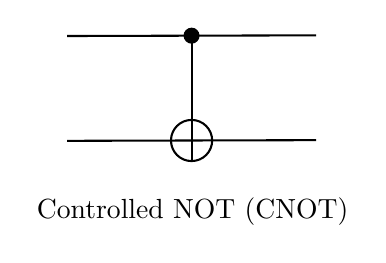
\begin{tikzpicture}[x=0.75pt,y=0.75pt,yscale=-1,xscale=1]
%uncomment if require: \path (0,300); %set diagram left start at 0, and has height of 300

%Straight Lines [id:da37432740726373037] 
\draw    (190,100) -- (310,99.67) ;


%Straight Lines [id:da2228128852300788] 
\draw    (250,99.83) -- (250,150.33) ;

\draw [shift={(250,99.83)}, rotate = 90] [color={rgb, 255:red, 0; green, 0; blue, 0 }  ][fill={rgb, 255:red, 0; green, 0; blue, 0 }  ][line width=0.75]      (0, 0) circle [x radius= 3.35, y radius= 3.35]   ;
%Shape: Circle [id:dp7117673469492589] 
\draw  [line width=0.75]  (240.08,150.33) .. controls (240.08,144.86) and (244.52,140.42) .. (250,140.42) .. controls (255.48,140.42) and (259.92,144.86) .. (259.92,150.33) .. controls (259.92,155.81) and (255.48,160.25) .. (250,160.25) .. controls (244.52,160.25) and (240.08,155.81) .. (240.08,150.33) -- cycle ;
%Straight Lines [id:da026806271903653256] 
\draw    (250,150.33) -- (250,160.25) ;


%Straight Lines [id:da8771832857323554] 
\draw    (190,150.5) -- (310,150.17) ;



% Text Node
\draw (250.5,184.5) node  [align=left] {Controlled NOT (CNOT)};


\end{tikzpicture}
\end{center}